\begin{frame}
  \frametitle{\textbf{$b$-jet Indetification}}
  \begin{columns}
    \column{0.5\textwidth}
    \begin{itemize}
    \item Many reconstructed objects can be used to discriminate between $b$ and light-jets
      \begin{itemize}
      \item Tracks
      \item Vertices
      \item Leptons
      \end{itemize}
    \item Combined-secondary-vertex (CSV) discriminator
      \begin{itemize}
      \item Combines vertex (and secondary vertex) information with track-based lifetime info in a complicated algorithm
      \item $b$-jets tend to contain secondary vertices
      \item Succeeded by \textit{DeepCSV}, a neural-network-based discriminator
      \end{itemize}
    \item \textbf{Muon rel-}$\boldmath{p_{\text{T}}}$
      \begin{itemize}
      \item Measures muon's transverse momentum relative to jet-axis
      \item $b$-quarks tend to impart more transverse momentum into daughter muons
      \end{itemize}
    \end{itemize}
    \column{0.5\textwidth}
    \centering
    \begin{tikzpicture}
      \node{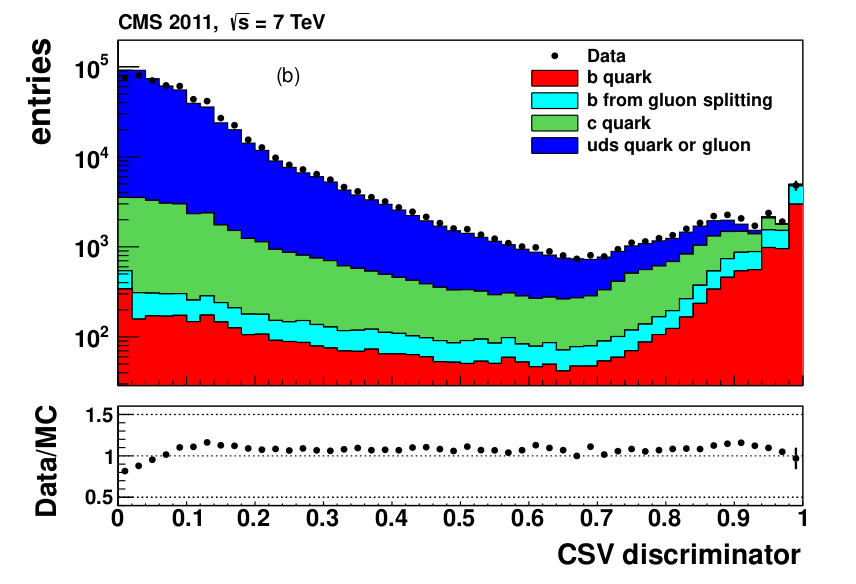
\includegraphics[width=0.68\textwidth]{csv-discriminator.png}};
    \end{tikzpicture}

    \
    
    \only<1>{
      \begin{tikzpicture}
        \node{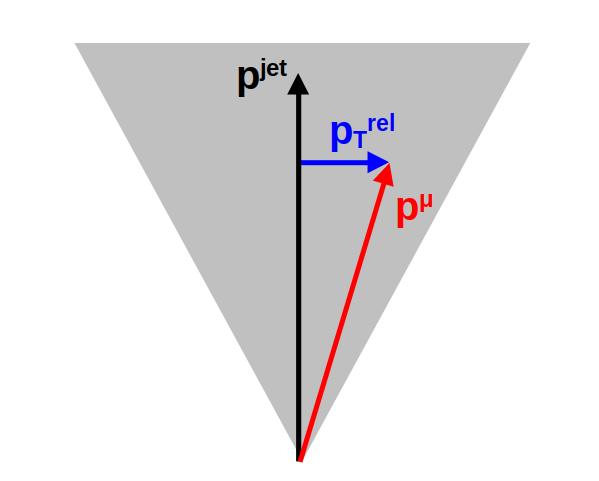
\includegraphics[width=0.65\textwidth]{pt-rel-cartoon.png}};
      \end{tikzpicture}
    }
    \only<2>{
      \begin{tikzpicture}
        \node{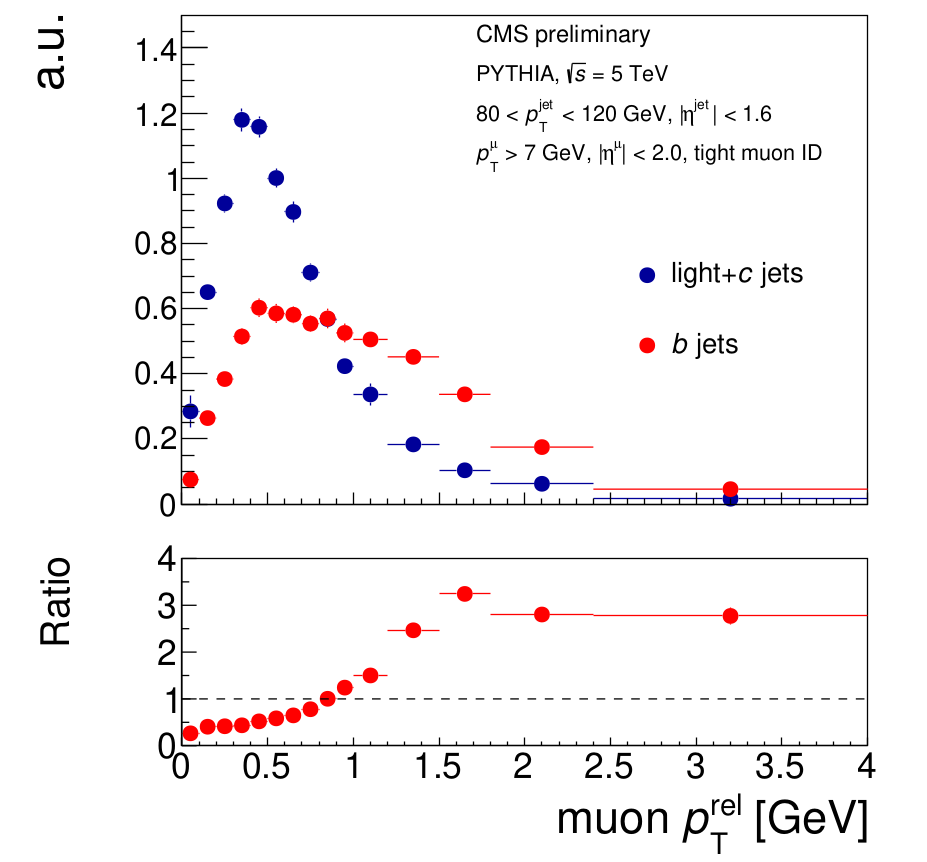
\includegraphics[width=0.68\textwidth]{muon-rel-pt.png}};
      \end{tikzpicture}
    }
  \end{columns}
\end{frame}
